\section{设计过程}
\subsection{设计流水账}
\textcolor{black}{

2024 年 12 月 25 日 12:30 \sim 15:30\\
到教室上课,听助教讲解硬件综合设计课程的大致规划和任务目标。

2024 年 12 月 25 日 12:30 \sim 15:30\\
配置了 vivado 2020.1 的环境,并将 vivado 的编辑器连接到了 vscode,这样可以获得更清晰的代码高亮和补正。并选择 lab4 代码作为我们小组的初版代码,将其代码连接到了资料包中的 lab4 工程并成功运行。剩下的时间开始各自学习重庆大学硬件综合设计实验文档的内容,修改代码。

2024 年 12 月 26 日 12:30 \sim 15:30\\
邹正强与罗梓元 添加了逻辑运算指令和移位指令。

2024 年 12 月 28 日 12:30 \sim 15:30\\
邹正强 添加了数据移动指令,小组一起讨论了 hilo 寄存器的放置位置,最终决定将其放置在 MEM流水线级。

2024 年 12 月 30 日 12:30 \sim 15:30\\
黄优文添加了算术运算指令。注意到拓展任务中的除法器的优化,小组开始查阅资料,寻找优化除法器的方法。

2024 年 12 月 31 日 12:30 \sim 15:30\\
黄优文添加了分支跳转指令。
 
2025 年 1 月 1 日 12:30 \sim 15:30\\
罗梓元添加了访存指令。

2025 年 1 月 2 日 12:30 \sim 15:30\\
邹正强连接了 sram-soc 运行功能测试,发现参考代码中的除法器不能通过功能测试中的除法,经过调试后通过,同时也解决了一些其他冒险模块的 bug 后通过功能测试的大部分测试点。

2025 年 1 月 3 日 12:30 \sim 15:30\\
小组观看了前几届学长录制在 B 站的视频,学习了异常处理有关的知识和注意事项,讨论了异常处理的相关设计思路,小组决定直接调用参考代码中的 cp0。

2025 年 1 月 4 日 12:30 \sim 15:30\\
黄优文完成了异常处理相关的数据通路的添加,开始调试。罗梓元完成了 cp0 相关数据通路的添加,开始调试。

2025 年 1 月 5 日 12:30 \sim 15:30\\
小组在与其他小组互相交流调试心得后,完成了代码的进一步调试。

2025 年 1 月 6 日 12:30 \sim 15:30\\
小组观看了 B 站学长的视频,准备开始连接 axi 总线,但是发现本次实验的资料包中没有提供相关的转接口代码,为了加快进度避免重复的工作,决定复用计算机组成与结构实验 5 的接口代码。

2025 年 1 月 7 日 12:30 \sim 15:30\\
邹正强连接好 axi 总线后开始测试 axi 项目的功能测试。 发现优化后的除法器不能通过部分测试点,黄优文开始修改除法器,最后通过了功能测试。

2025 年 1 月 8 日 12:30 \sim 15:30\\
决定采用罗梓元 的 cache 代码来进行后续的开发。连接了计组实验 5 中编写的 写回 cache,成功通过性能测试并上板得到了性能得分,并继续优化 cache。

2025 年 1 月 9 日 12:30 \sim 15:30\\
在确定代码的大致通路后,邹正强开始用 Viso 绘制数据通路图。罗梓元 与 黄优文开始编写部分报告内容。罗梓元 替换二路组相联写回cache 后发现上不了板,最终决定采用原来的写回cache。

2025 年 1 月 10 日 12:30 \sim 15:30\\
小组现场添加指令和答辩。

2025 年 1 月 11 日 12:30 \sim 15:30\\
小组撰写剩余的报告内容。
}

\subsection{错误记录}

\subsubsection{错误1}
\begin{enumerate}[(1)]
    \item 错误现象:\textcolor{black}{ CPU 功能测试 jr 报错}
    \item 分析定位过程:\textcolor{black}{ 首先我们发现它一条 jump and link 类型的指令,它会导致 pc 的跳转, pc 跳转会和下图中的 7 个信号值有关,现在把这些信号值全部拉出来对比,查看哪一步信号值跳转出错。 从图中可以看到 JrD 信号为 1 时,alu 的计算结果还没有到达,所以这里需要阻塞一个周期的流水线,等待结果传入,然后由 ForwardAD进行数据前推。需要在 hazard 模块中添加一个阻塞信号 jrinstallD。
}
    \item 错误原因:\textcolor{black}{ 添加 jr 型指令后没有修改 hazard 模块,需要添加相关类型的阻塞信号}
    \item 修正效果:\textcolor{black}{ 在添加了 jr 阻塞信号后,jr 指令阻塞了一个周期,获得了正确的数据前推值,完成了跳转。}
    \item 归纳总结:\textcolor{black}{ 这个错误的出现是因为没有考虑到新加入的指令的冒险现象,由于经验较少,这类错误是无法避免的,只能在测试时及时发现,及时修改。}
\end{enumerate}

\subsubsection{错误2}
\begin{enumerate}[(1)]
    \item 错误现象:\textcolor{black}{CPU 功能测试 syscall 报错}
    \item 分析定位过程:\textcolor{black}{先分析如下错误波形图:这里的第一次执行 syscall 指令,跳转到0xbfc00380 执行异常处理。异常处理的第一条指令是从 hilo 寄存器中取值到另外两个寄存器。但是这里出错了,从波形图可以看出,出错的原因在于在异常处理跳转过后,hilo 寄存器的值被覆盖了,所以在这里需要为我们的 hilo 寄存器添加一个接口,用于阻塞 hilo 寄存器。
}
     \begin{figure}[htbp]
        \centering
        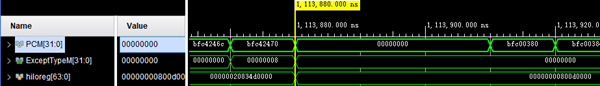
\includegraphics[width=\textwidth]{image/wave1.png}
        \caption{错误的波形图}
    \end{figure}
    
    \item 错误原因:\textcolor{black}{异常处理时hilo 寄存器没有被阻塞,导致值被刷新覆盖了。}
    \item 修正效果:\textcolor{black}{错误修改后的波形图如下所示:}
    \begin{figure}[htbp]
        \centering
        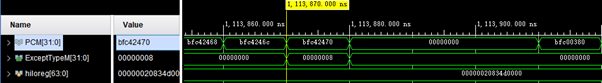
\includegraphics[width=\textwidth]{image/wave2.png}
        \caption{错误修改后的波形图}
    \end{figure}
\end{enumerate}

\subsubsection{错误3}
\begin{enumerate}[(1)]
    \item 错误现象:\textcolor{black}{综合阶段出现下面错误:
    [Place 30-4] Design utilization is very high. Run report\_utilization command to see design utilization}
    
    \item 分析定位过程:\textcolor{black}{这个bFPGA或ASIC设计的放置阶段,表示设计的资源利用率过高,导致放置操作不太可能成功}
    \item 错误原因:\textcolor{black}{二路组相联cache 消耗资源比直接映射大导致实现阶段实现不了}
    \item 修正效果:\textcolor{black}{资源消耗过大}
    \item 归纳总结:\textcolor{black}{使用普通的写回cache 即可}
\end{enumerate}

\subsubsection{错误4}
\begin{enumerate}[(1)]
    \item 错误现象:\textcolor{black}{两路组相联写回cache 一个组里只有第一个缓存行会存数据,另外一个一直为未知值,错误如下图所示。}
    
    \begin{figure}[htbp]
        \centering
        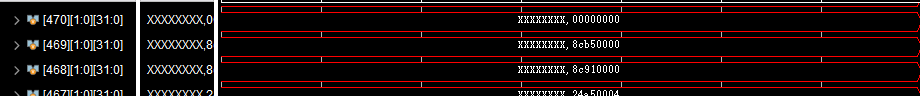
\includegraphics[width=\textwidth]{image/errorcache.png}
        \caption{cache错误波形图}
    \end{figure}
    
    \item 分析定位过程:\textcolor{black}{写入 cache 时判断一组内两个缓存行是否有数据或者是否命中的逻辑出现问题}
    \item 错误原因:\textcolor{black}{判断逻辑出错}
    \item 修正效果:\textcolor{black}{修改代码后正确效果如下图所示:}
    \begin{figure}[htbp]
        \centering
        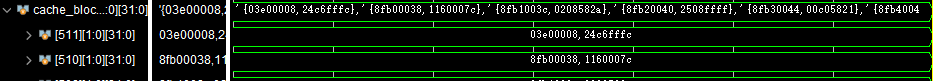
\includegraphics[width=\textwidth]{image/cachesuccess.png}
        \caption{cache正确波形图}
    \end{figure}
\end{enumerate}

\subsubsection{错误5}
\begin{enumerate}[(1)]
    \item 错误现象:\textcolor{black}{功能测试 CP0 报错}
    \item 分析定位过程:\textcolor{black}{先来看错误的波形图,波形图中可以看到出现问题的原因是刷新信号提前出现了,在下个周期到来了之前,cp0 已经写入了 PCM 的值,导致需要的 PCM 的值比预期的少 4。这是由于 stall\_all 信号并没有暂停 cp0 的工作,现在需要给 cp0也接入阻塞信号,阻塞它在等待访存数据阶段的写入操作。}
    
    \begin{figure}[htbp]
        \centering
        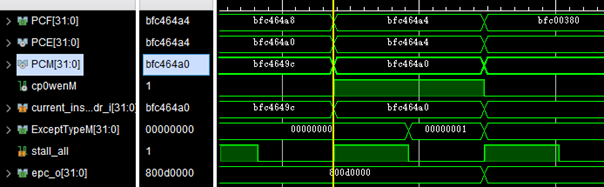
\includegraphics[width=0.65\textwidth]{image/wave3.png}
        \caption{错误的波形图}
    \end{figure}
    
    \item 错误原因:\textcolor{black}{cp0 没有接入控制冒险。}
    \item 修正效果:\textcolor{black}{修改过后正确的结果如下所示:}
    \begin{figure}[htbp]
        \centering
        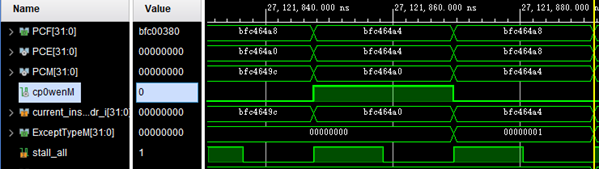
\includegraphics[width=0.65\textwidth]{image/wave4 (2).png}
        \caption{错误修改后的波形图}
    \end{figure}
\end{enumerate}

\subsubsection{错误6}
\begin{enumerate}[(1)]
    \item 错误现象:\textcolor{black}{功能测试 bfc423a8: 269423ac addiu s4,s4,9132 报错。}
    \item 分析定位过程:\textcolor{black}{出问题的指令是异常处理的第一条指令,出现异常的原因是在异常处理的时候如果阻塞了信号,会刷新所有流水线寄存器,导致结果指令丢失。}
    \item 错误原因:\textcolor{black}{在异常处理的时候如果阻塞了信号,会刷新所有流水线寄存器,导致结果指令丢失。}
    \item 修正效果:\textcolor{black}{在所有的刷新信号上和∼stall\_all 做与运算,这样就可以在阻塞时不刷新流水线寄存器。}
\end{enumerate}

\subsubsection{错误7}
\begin{enumerate}[(1)]
    \item 错误现象:\textcolor{black}{功能测试 bfc3a8cc: 0000a812 mflo s5 报错}
    \item 分析定位过程:\textcolor{black}{先来分析错误的波形图:从图中可以看到 hilo 寄存器的值在 EX 级就可以取到了,之后步步提前了一个周期,导致错误。既然提前了一个周期,那么可以放入流水线寄存器中多存一个周期,就可以得到正确的结果了。}
    
    \begin{figure}[htbp]
        \centering
        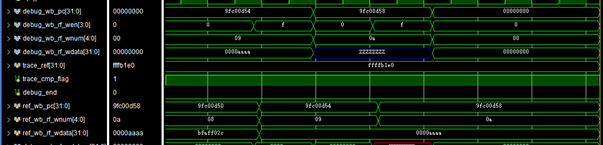
\includegraphics[width=\textwidth]{image/wave5.png}
        \caption{错误的波形图}
    \end{figure}
    
    \item 错误原因:\textcolor{black}{hilo 寄存器没有被 stall\_all 信号阻塞。}
    \item 修正效果:\textcolor{black}{在流水线寄存器中多存一个周期,就可以得到正确的结果。}
\end{enumerate}